Since the 1970s \parencite{article14}, the decade in which the microprocessor era started, the overall performance of a processor has increased \parencite{inproceedings4}. This goal was achieved by several points, including ``\textit{sophisticated process technology, innovative architecture or micro-architecture}'' \parencite[see][Chapter 1, p2]{inproceedings4}. In fact, increasing the clock speed of a single core processor, like Moore's Law predicted \parencite{article14}, was usually reached by increasing the number of transistors on the chip \parencite{article14}. However, this go along side with the increase in complexity \parencite[see][Pollack’s rule]{article14}, which mean, that doubling the logic of a processor result in a performance boost of only 40\% \parencite[see][Chapter 2]{article14}.

Another huge problem chip manufacturers have to deal with is leakage power \parencite[see][Chapter 2, p3]{inproceedings4}, because the ``\textit{transistor leakage current increases as the chip size shrinks}'' \parencite[see][p2]{article14} [see Chart \ref{fig:leackagePer}]. An increase of leakage current of the transistors also result in a increase of the die's temperature \parencite{inproceedings4} along side the total power consumption as well.
\begin{figure}[h!]
	\centering
	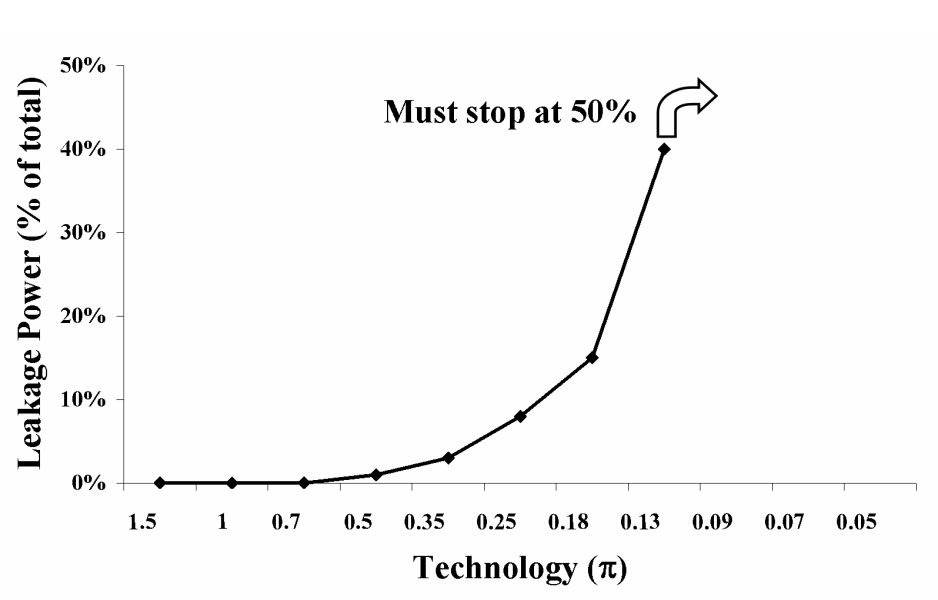
\includegraphics[scale=0.25]{leackage-power_vs_process-technology.png}
	\caption{
		Leakage Power (\% of total) vs. process technology \parencite{inproceedings4}
	}
	\label{fig:leackagePer}
\end{figure}

Furthermore, a increase of the processor clock frequency to speed up the performance is only available to a suffisticating limit of 4GHz \parencite{article14}. After this frequency threshold, also known as reaching the power wall, the ``\textit{power dissipation}'' \parencite[see][p2]{article14} increases again.

Facing these types of problems such as ``\textit{chip fabrication costs, fault tolerance, power efficiency, heat dissipation}'' \parencite[see][p3]{article14} along side with increasing processor performance, the only possible solution chip manufacturers and companies could offer was parallelism. 

\newpage

\section{Basic Concept}

Parallelism for processing is not something new. But due to the fact that real thread level parallelism [see Chapter \ref{subchap:threadLevelParallelism}] was only available after dual or multi-core processors were invented in 2005 \parencite{internet6}, the topic itself and efficient software implementations are still treated in scientific work \parencite{book3} \parencite{article2}.

\begin{figure}[h!]
	\centering
	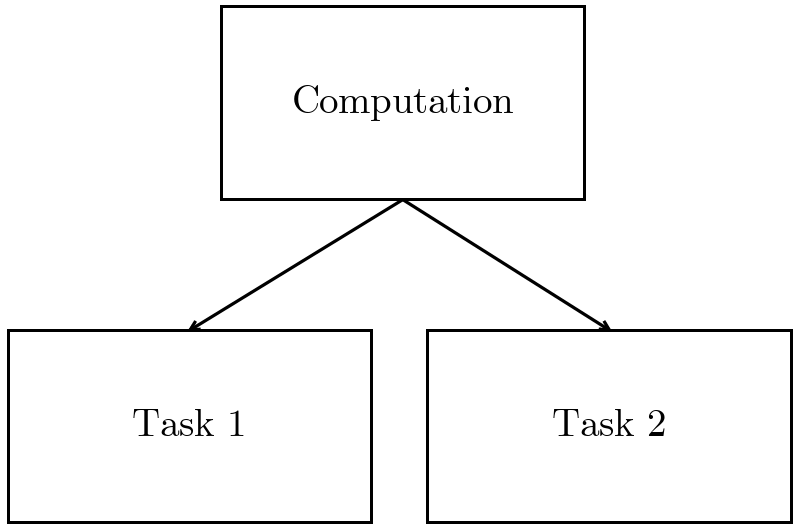
\includegraphics[scale=0.3]{basic-parallelism.png}
	\caption{
		The basic concept of a simple concurrency computation.
	}
	\label{fig:basicPara}
\end{figure}

In general, parallelism for programming means to split up a task or a computation into several sub tasks [e.g. Figure \ref{fig:basicPara}] or results, to decrease the execution time. Depending on the problem itself, these separated tasks can be independent or connected [see Chapter \ref{chap:parallelPrinciples}]. If we want to talk about the general concept of parallelism, we have to take a closer look to some mathematical laws, which try to describe the availability to parallel task execution and their limits.

\subsection{Amdahl's Law}

The first one, which quantifies parallelism, is called Amdahl's Law \parencite{inbook1}. During the publication period of Amdahl's paper \parencite{book6}, critics claimed ``\textit{that the organization of a single computer has reached its limits and that
truly significant advances can be made only by interconnection of a multiplicity of computers}” \parencite[see][p80]{inbook1}. Of course this can be transferred on single and multi-core processors or even on multi threading \parencite[see][Chapter 1.3, p2]{phdthesis1}, but in fact, like Amdahl claimed too, addressing hardware \parencite{inbook1}, and nowadays switching context time was not considered in this case.

Amdahl's Law wants ``\textit{to provide an upper limit on speedup}'' \parencite[see][p81]{inbook1} in general to point out that there is a overhead \parencite{inbook1}, which can not pe implemented in parallel, but at the same time, ``\textit{apart from the sequential fraction, the remaining computations are perfectly parallelizable}'' \parencite[see][p81]{inbook1}.

\newpage

\begin{figure}[h!]
	\centering
	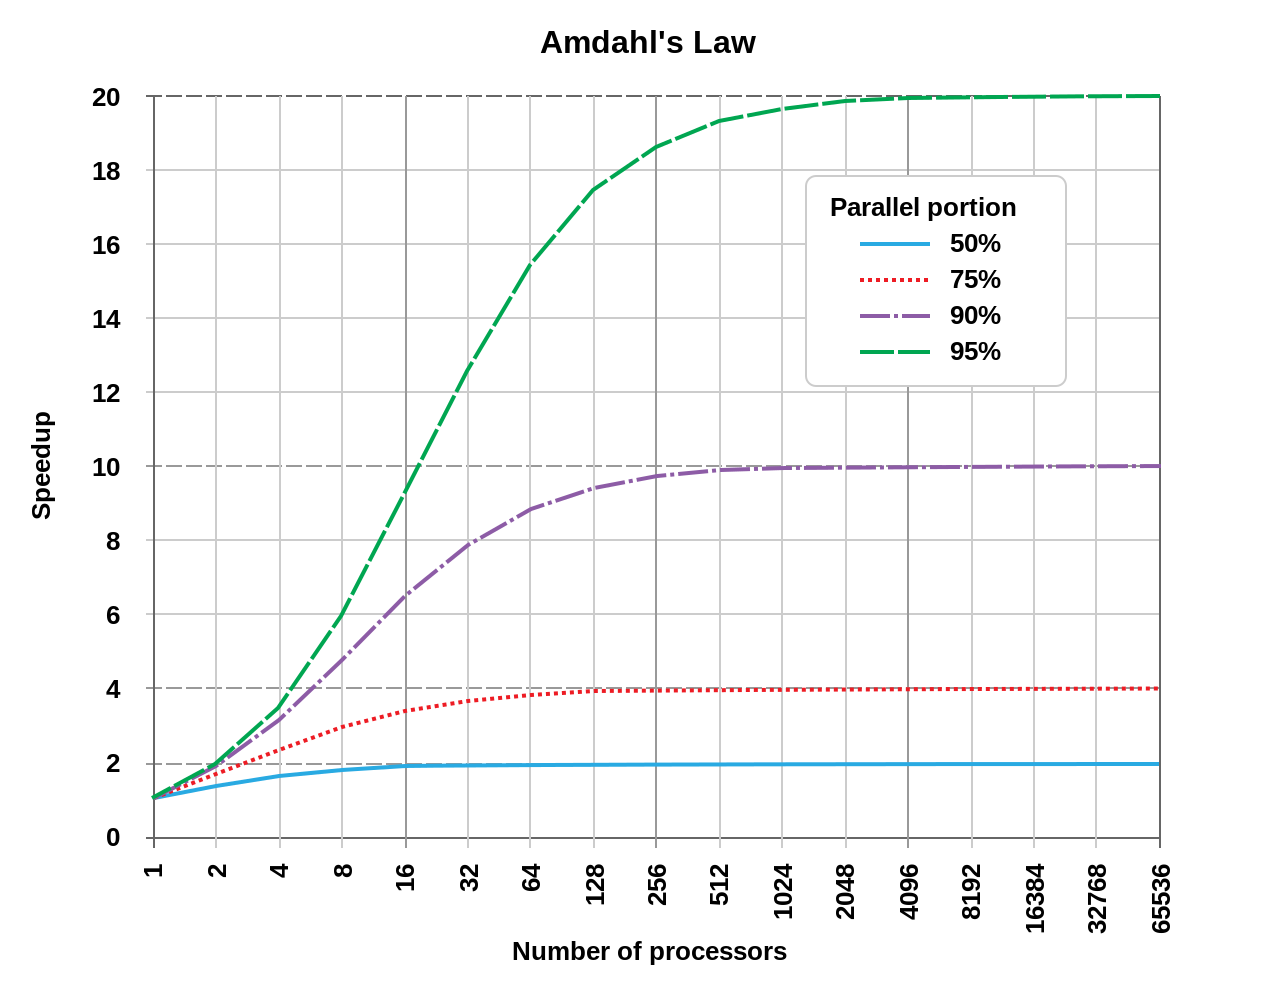
\includegraphics[scale=0.95]{amdahls-law.png}
	\caption{
		The limited speed-up of a program, which can be parallelized, depending on the number of parallel executions \parencite{image1} \parencite[similar to][p4]{phdthesis1}.
	}
	\label{fig:admLaw}
\end{figure}

\noindent So regarding to Amdahl's Law, there has to be an upper limit of parallelism, due to the fact, that some sequential fractions still exists. In order to be able to describe this relationship, the time required to perform a calculation at once is related to the total time in parallel execution:

``\textit{Let t\textsubscript{1} be the time taken by one processor solving a computational problem and t\textsubscript{p} be the time taken by p processors solving the same problem. Finally let us denote the supposed inherently sequential fraction of instructions by f. Then, according to Amdahl, t\textsubscript{p} = t\textsubscript{1}(f+(1-f)/p) and the speedup obtainable by p processors can be expressed as}'' \parencite[see][p81]{inbook1}:

\begin{equation} \label{formula:amd}
	s = \frac{t_1}{t_p} = \frac{1}{f + (1 - f) / p}
\end{equation}
\\[2pt]
For example, a program which contains 90\% of parallelizable code [see Figure \ref{fig:admLaw}] reaches his speed up limit at around 512 cores [formula  \ref{formula:amdLimes}]; in this case we substitute f= 0.2/2. After that number of processor cores, an significant speed up increase is not noticeable anymore . 

\begin{equation} \label{formula:amdLimes}
	\lim_{p \to \infty f \to 0.1} \left( \frac{t_1}{t_p} \right) = \lim_{p \to \infty} \left( \frac{1}{0.1 + (1 - 0.1) / p} \right) = 10
\end{equation}
\\[2pt]
Many other authors tried to claim that this upper limit of speed up, both in theory and practice, is not the final end. To proof that, only to mention a few , they took into account the ``\textit{energy per instruction (EPI)}" \parencite[Annavaram et al. in][Chapter 3,  p81]{inbook1}, a case study depending on ``\textit{asymmetric (or heterogeneous) chip multiprocessor architectures}'' \parencite[Kumar et al. in][Chapter 3,  p81]{inbook1} or even considering ``\textit{disk arrays to reduce input-output requirements}'' \parencite[Patterson et al. in][Chapter 3,  p81]{inbook1}.

\newpage

\subsection{Gustafson’s Law's}

Due to the fact that Gustafson’s Law's is based on ``\textit{the same concepts as the
bases of Amdahl’s law, it is more a variant, rather than a refutation}'' \parencite[see][p81]{inbook1}. But in fact, it is another mathematical consideration, which offers, in comparison to Amdahl's Law, no upper speed up limit regarding parallelism. Related to Gustafson, the time a single core processor needs solving the same computational problem on the sequential would be \textit{ft\textsubscript{p}}, and on the parallelizable part \textit{(1-f)pt\textsubscript{p}}. Therefore, the total amount of achievable speed up by p processors can thus be calculated

\begin{equation} \label{formula:gustLaw}
	s = \frac{t_1}{t_p} = \frac{ft_p + (1 - f)pt_p}{t_p} = f + (1 - f)p
\end{equation}
\\[2pt]
using the formula \ref{formula:gustLaw} above. In this case, ``\textit{f is the same “inherently sequential” fraction of instructions as in the case of Amdahl’s law}'' \parencite[see][p81]{inbook1}. In addition to that, he doesn't take the ``\textit{sequential input-output requirements proportional to input and output sizes into account}'' \parencite[see][p81]{inbook1}.

\begin{figure}[h!]
	\centering
	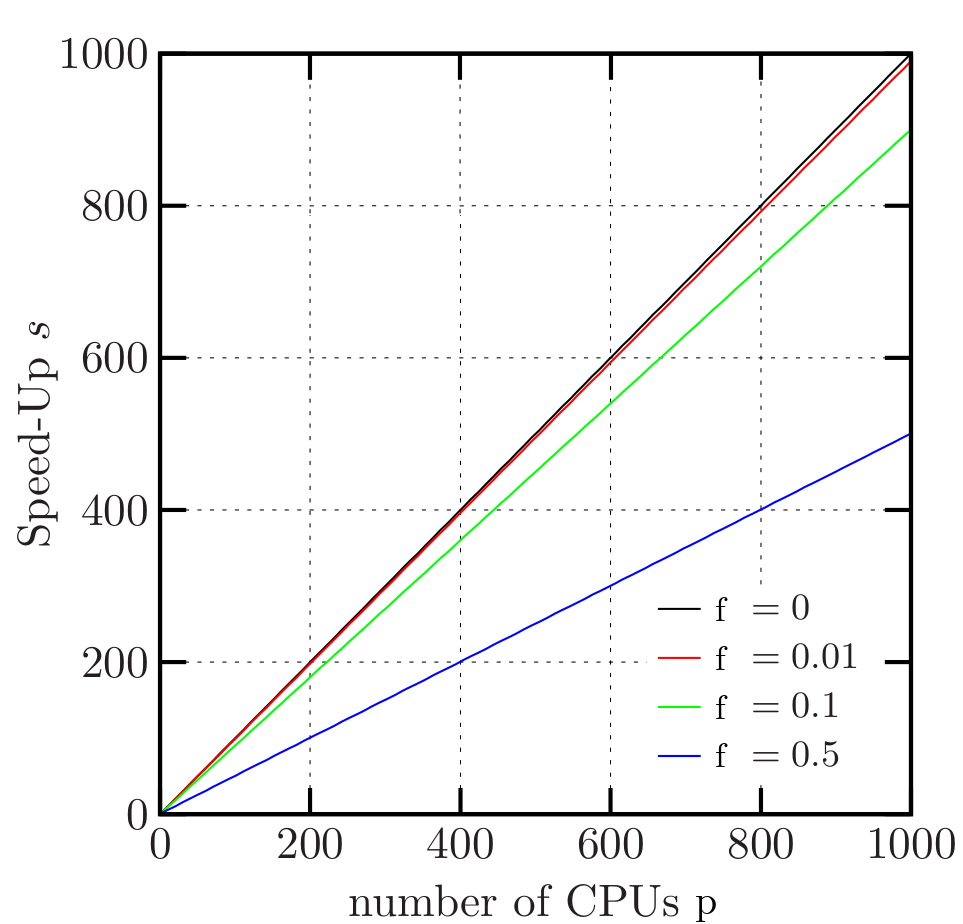
\includegraphics[scale=0.28]{gustafssons-law.png}
	\caption{
		Gustafson’s Law. In contrast to Amdahl we now have no upper limit to the speed up. \textit{f} only determines the slope of the speed-up \parencite{article19}.
	}
	\label{fig:gustLaw}
\end{figure}

Regarding to \parencite{inbook1}, neither Amdahl's or Gustafson’s Law are suitable to quantify parallelism in theory and practice, because both don't take into account, that ``\textit{sequential fractions of computations have negligible effect on speedup if the growth rate of the parallelizable fraction is higher than that of the sequential fraction}'' \parencite[see][Chapter 7, p88]{inbook1}.

Furthermore, \parencite{inbook1} point out, that no simple formula governing parallelism exists. Both laws are more of an attempt to describe experimental results, and therefore understood rather as a draft rule of thumb as a law.

\newpage

\subsection{Principles of Parallel Computing}\label{chap:parallelPrinciples}

Despite trying to quantify the ability to parallelism task processing, it is also important to keep in mind the basic aim of parallelism to mention a ``\textit{design for concurrency}'' \parencite[see][p4]{article6}. First of all, reducing the execution time is one of the most important objective in concurrency to make applications more \textbf{efficient}. Computations, and even tasks, are getting more and more complicated \parencite{internet2}, not only in the application field of scientific researches. Today's software applications require sophisticated hardware like multi-core processors, to offer a suitable user experience, for example in gaming (e.g VR), augmented reality in automation (e.g. AR) or for IoT [see Chapter \ref{chap:introduction}] devices.

\begin{figure}[h!]
	\centering
	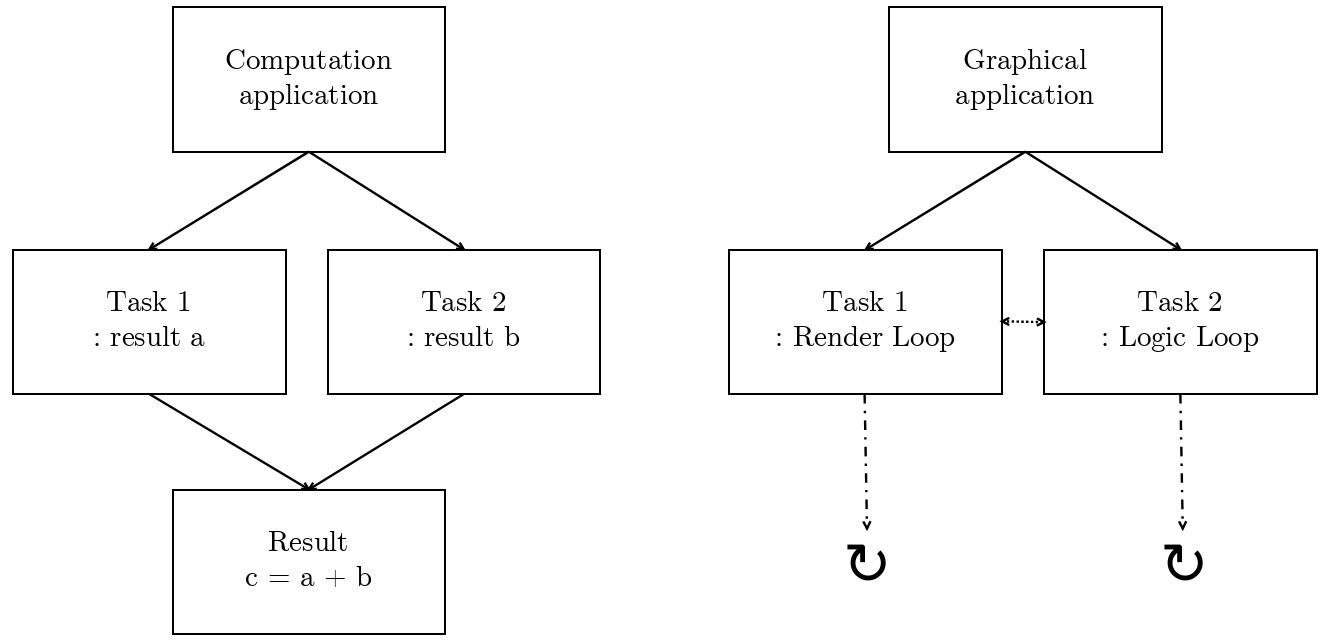
\includegraphics[scale=0.32]{comparison-comp-indep-par-depnd-par.png}
	\caption{
		Comparison of independent and dependent tasks in a general concurrency application.
	}
	\label{fig:compIndeDepConcurr}
\end{figure}

In case of software parallelism, which is the main objective of this chapter, we have to distinguish between tasks, which are independent and tasks, which are connected (called dependent). It depends largely on the application itself: e.g. for example, a numerical calculation [see Chapter \ref{chap:mathComp}] can be easily subdivided into sub tasks to speed up the computation, whereas a graphical application needs a logical loop and a render loop, both independently in different tasks [see Fig. \ref{fig:compIndeDepConcurr}]; a data exchange usually takes place via a shared memory [more on this in Chapter \ref{chap:parallelCompArch}]. As already suggested in Chapter \ref{fig:basicPara}, our work will be limited to the division of numerical or generic mathematical calculations. 

In addition to that, multi-core software applications offers also the opportunity, to provide low power systems, because \textbf{power consumption} results from performance and clock frequency \parencite[see][Fig. 3, p4]{article14}, along side instructions per core (IPC) \parencite{inproceedings4} [further inf. in Chapter \ref{chap:parallelprg}].

\newpage

\begin{figure}[h!]
	\centering
	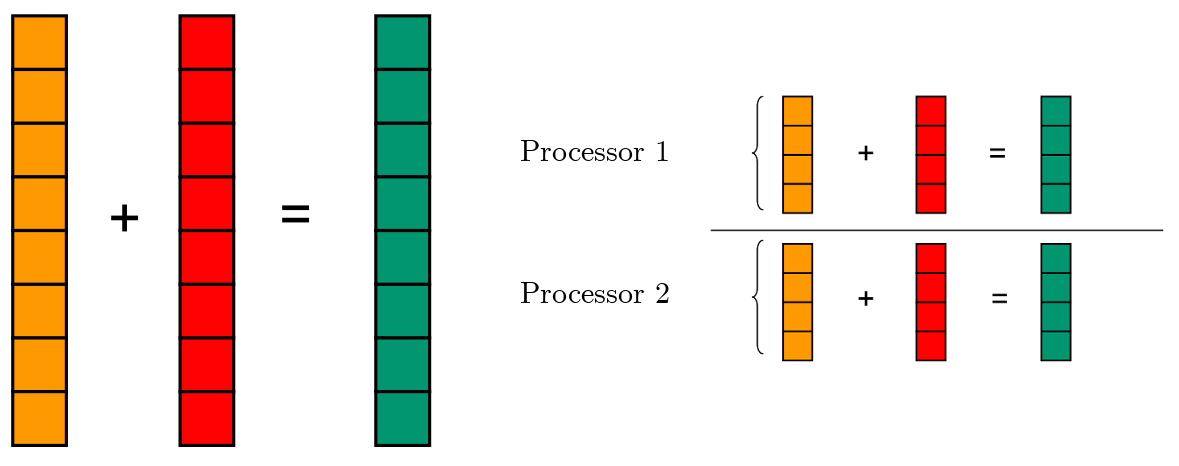
\includegraphics[scale=0.25]{array-split-parallelism.png}
	\caption{
		Adding to arrays of integers for speed up in concurrency \parencite[see][p3]{internet2}.
	}
	\label{fig:arraySplit}
\end{figure}

\noindent Furthermore, to guarantee \textbf{flexibility} for both, the software application and hardware platform, multi-core systems and concurrency is the way to go to fit customers and companies claims. This can easily be proofed due to the fact that today's hard- and software manufacturers always try to provide generalized solutions.   

It can not be denied that as the degree of parallelism increases, the complexity of the application including the hardware realization also increases \parencite{article14} \parencite{article6}. A basic principle and design pattern of parallel computing is therefore to ensure maximum efficiency through parallelism while reducing complexity. A usual rule can be transferred on this topic: ensure \textbf{simplicity}.

Regarding to Figure \ref{fig:compIndeDepConcurr} and Chapter \ref{chap:mathComp}, the best way to implement and computation concurrent is to guarantee that the sub tasks can work independent from each other. This has a major effect on the performance and complexity of the software implementation: ``massively parallel vs. embarrassingly serial'' \parencite[see][p15]{article6}, alongside the ability to take less attention on control issues such as task orders, synchronization, (shared) memory access or even task communication \parencite{internet1}. In fact, complete concurrency is not possible, due to the fact that splitting a computation into sub tasks requires at least on remaining worker task to collect and combine the sub task results. Anyway, \textbf{Independence} of sub tasks enables almost the best efficiency.\\

\noindent \textbf{Emphasises design}  \parencite[see][p5]{article6}: In summary, therefore, the following points should be seen as goals and thus as groundbreaking for the basic principles of parallelism:

\begin{enumerate}
	\item \underline{Efficiency}: 
	
	Concurrency in hard- and software to solve large problems in less amount of time to reduce execution time and power consumption.
		
	\item \underline{Flexibility}: 
	
	Environments will be more heterogeneous and the use in different application areas will be enabled.
	
	\item \underline{Simplicity}:
	
	Code for Parallel Computing will be more complicated, because synchronization or memory access have to be regulated. One reason more ``\textit{to strive for maintainable,
	understandable programs}'' \parencite[see][p6]{article6}. 
	
	\item \underline{Independence}:
	
	To ensure maximum efficiency, parallel computations should be independent.
\end{enumerate}

\newpage

\noindent These principles result in four different \textbf{design patterns} \parencite[see][p11 ff.]{article6} for parallel software applications:
\begin{itemize}
  \item \underline{Finding concurrency}: 
  
  This should be the main aim of all software applications today, set the case it makes sense.
    \item \underline{Algorithm structure}: 
  
  To ensure proper efficient, the implementation should be based on usual parallel programming models [see Chapter \ref{chap:parPrgModels}].
  
  \item \underline{Supporting structures}: 
  
  ``\textit{Useful idioms rather than unique implementations}'' \parencite[see][p25]{article6} like Loop Parallelism, Fork/Join, Shared Data or Shared Queue \parencite{article6}.
  
  \item \underline{Implementation Mechanism}: 
  
  Using programming languages which offer the opportunity to real parallel computing (e.g. C++, OpenMP \& Pthreads, MPI, OpenCL) \parencite{article6}.
  
\end{itemize}

\section{Definition of parallel mathematical computations}\label{chap:mathComp}

We talked about how to quantifying parallelism, and above that, also about the principles of parallel computing and the resulting design patterns for parallel computing. Now its time to take into account the necessary mathematical computations. Not all calculations are suitable for parallelism, so we have to work out properties for the quantification of possible numerical or mathematical methods. 

\begin{equation} \label{formula:scalarVec}
\vec{a} = \begin{bmatrix}
a_{0} \\
a_{1} \\
\vdots \\
a_{i} \\
\vdots \\
a_{N - 1} \\
\end{bmatrix} ,\quad \vec{b} = \begin{bmatrix}
b_{0} \\
b_{1} \\
\vdots \\
b_{i} \\
\vdots \\
b_{N - 1} \\
\end{bmatrix}
\end{equation}

The easiest way to do that is to take a look at two basic examples. The first one will be a simple scalar product of two \textit{N} dimensional vectors $\vec{a}$ and $\vec{b}$ [see formula \ref{formula:scalarVec}]. Both vectors have the same dimension \textit{N} and are not orthogonal to each other; otherwise the scalar product would be very simple to calculate and the result null, regardless of the dimension of the vectors. The scalar product of two N dimensional vectors are defined as

\begin{equation} \label{formula:scalarProdEasy}
	s = \vec{a} \cdot \vec{b} = a_0 \cdot b_0 + a_1 \cdot b_1 + \quad \cdots \quad + a_{N - 1} \cdot b_{N - 1}
\end{equation}

\noindent or more formally like

\begin{equation} \label{formula:scalarProd}
	s = \sum_{i=0}^{N - 1} a[i] \cdot b[i]
\end{equation}

\newpage

As mentioned in formula \ref{formula:scalarProdEasy}, theoretically any kind of scalar product can be easily calculated in parallel using \textit{N} processor cores or tasks. We even don't have to take care about accessing resources, because all tasks will use their one values depending on the index elements of the vectors. Only in the end, the final result has to be calculated including the results, which are returned from the different tasks.

But to keep it simple, we will only separate the given scalar product [see formula \ref{formula:scalarProd}] into to different tasks. A synonymous representation would be the following:

\begin{align} \label{formula:scalarProdSeq}
	\begin{aligned}
		s &= \sum_{i = 0}^{N / 2 - 1} \left(a[i] \cdot b[i]\right) + \sum_{i = N / 2}^{N - 1} \left(a[i] \cdot b[i]\right)
		\\ &=  \underbrace{\sum_{i = 0}^{N / 2 - 1} \left(a_{local}[i] \cdot b_{local}[i]\right)}_\text{p\textsubscript{0}} \qquad \vertarrowbox{+}{process communication} \qquad \underbrace{\sum_{i = N / 2}^{N - 1} \left(a_{local}[i] \cdot b_{local}[i]\right)}_\text{p\textsubscript{1}}
	\end{aligned}
\end{align}

The important sign in formula \ref{formula:scalarProdSeq} is the ``+''. It seems inconspicuous, but in fact, this is the the one we have to take care about most. The ``+'' symbol indicates required ``communication between the processes'' \parencite[see][p]{internet2} p\textsubscript{0} and p\textsubscript{1}. So the essential part in every parallel computation will be collecting the sub results together. This could either be achieved by returning each result from the sub task to the main task or storing the sub result locally in memory, so it can be collected afterwards.

The complex theory would categorize this kind of computation as a decision problem in the \textit{NC} class as a subset of \textit{P} \parencite{book8}. In general, all computations are stored in the \textit{P} class of decisions. \textit{NC} problems ``\textit{can be solved in parallel time (log n)\textsuperscript{O(1)} using n\textsuperscript{O(1)} processors}'' \parencite[see][Chapter 10, p91]{inbook1}. In other words, \textit{NC} problems can be solved in ``\textit{polylogarithmic time by using a polynomial number of processors}'' \parencite[see][Chapter 10, p91]{inbook1}. Furthermore they are also known as fast parallel working algorithms \parencite{inbook1} and in most of the cases as the most efficient ones \parencite{book8}.\\

\noindent In comparison to a almost perfectly independent parallel computations, the question arises, whether a ``inherently sequential'' problem exists. This type of computations, due to the complex theory, belong to the class of \textit{P-complete} \parencite{inbook1} decisions and are also known as difficult to parallelize effectively or being solved in limited space. Regarding to \parencite{inbook1}, no ``real'' \textit{P-complete} problems exists, and considered to \parencite{book8}, sequential models are in fact parallelizable, but this comes ``\textit{at the cost of an enormous number of processors}'' \parencite[see][Chapter 5.5, p69]{book8}, resources or even execution time \parencite[see][p61]{book8}.

So lets take a look at our second example, which might seems easily to compute, but in fact comes with a major bottleneck if we are trying to solve this kind of problem in parallel. The best known mathematical calculation to illustrate this is the prefix sum \parencite{article7}. Let's say we have a vector with N elements like mentioned underneath [see formula \ref{formula:prefixVec}]:

\begin{equation} \label{formula:prefixVec}
\vec{x} = \begin{pmatrix}
	x_{0} & x_{1} \quad \cdots \quad x_{i} \quad \cdots \quad & x_{N - 1} \\
\end{pmatrix}
\end{equation}

\newpage

The prefix sum is defined as a partial sum of series of each the vector elements. A none formally expression is shown in the following formula [see \ref{formula:prefixSumNonFormal}].

\begin{align} \label{formula:prefixSumNonFormal}
	\begin{aligned}
	y_0 &= x_0 \\
	y_1 &= x_0 + x_1 \quad &= y_0 + x_1 \\
	y_2 &= x_0 + x_1 + x_2 \quad &= y_1 + x_2 \\
	\vdots \\
	y_i &= y_{i - 1} + x_i \\
	\end{aligned}
\end{align}
\\[2pt]
It is obvious that the prefix sum can be easily calculated in sequential with the last equation in [\ref{formula:prefixSumNonFormal}]. The resulting solution vector based on the input vector $\vec{x}$ [see formula \ref{formula:prefixVec}] should be represented in the following notation:\\

\begin{equation} \label{formula:prefixSumNonFormal}
	\vec{y} = \begin{pmatrix}
		x_{0} & x_{0} + x_{1} \quad \cdots \quad y_{i} \quad \cdots \quad & y_{N - 2} + x_{N-1} \\
	\end{pmatrix}
\end{equation}
\\[2pt]
To major problem with this computation is the fact, that each part result is dependent on the result before. A parallel computation is possible, but not like the implementation mentioned in [\ref{formula:scalarProdSeq}], because therefore no major decrease of execution time would be achieved. Indeed, there are some parallel solutions for the prefix sum, but with restrictions such as efficiency, span \parencite{article21} or less parallelism \parencite{article22}.

If we want to quantify parallel mathematical computation models, based on the examples which we worked out, the following three points should be taken into account:

\begin{enumerate}
	\item Divisibility of the calculation.
	\item Independence of the sub task calculations.
	\item Involvement of achievable work efficiency. 
\end{enumerate}

\newpage

\section{Parallel Computer Architecture}\label{chap:parallelCompArch}

The terminology of computer architecture was invented in 1960s by the designers of IBM System to describe the structure of a computer. Computer architect’s task is to write an suitable program code for the machine, keeping in mind every time this structure of computer, understanding all the factors like state-of-the-art technologies at each design level and changing those designs tradeoffs for their specific applications \parencite{article20}.

Parallel computing means the situation where tasks are separated into discrete parts that can be executed concurrently. Each part is diffused into a larger series of instructions which will be executed simultaneously on different CPU's or even in a pipeline [see Figure \ref{fig:parallelismPipe}]. These kind of parallel systems have to deal with the simultaneous use of multiple computer resources that can include either a single computer with multiple CPU's, or a number of computers connected by a network creating a parallel processing cluster or combination of both.

The crux of parallel processing are CPU's. Based on the number of instruction and data streams that can be processed simultaneously, computing systems are classified into four major categories based on Flynn’s Taxonomy \parencite{internet7}.

\begin{figure}[h!]
	\centering
	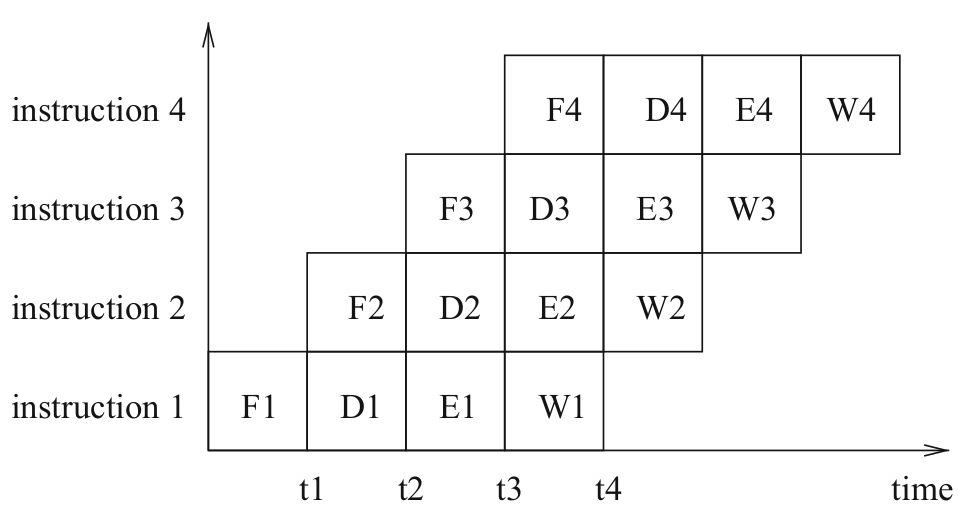
\includegraphics[scale=0.28]{parallelism-pipelining.png}
	\caption{
		Overlapping execution of four independent instructions by pipelining. The execution of each instruction is split into four stages: \textit{fetch (F)}, \textit{decode (D)}, \textit{execute (E)}, and \textit{write back (W)} \parencite[see][Fig. 2.1, p11]{book1}.
	}
	\label{fig:parallelismPipe}
\end{figure}

\subsection{Flynn's Taxonomy of Parallel Architectures}\label{subchap:flynnsTax}

Flynn’s classification was first elaborated and proposed by Michael Flynn in 1966 and represents a scheme which is based on the notion of information stream. The term ‘stream’ defines a sequence or flow of either one of both existent types of information which flows and are operated into a processor: instructions or data. 

Instruction stream defines the sequence of instructions performed by CPU, as in the same time the data stream defines the data traffic exchanged between the memory and CPU.His taxonomy left aside the machine’s structure for classification of parallel computers and took over a whole new concept focusing on multiplicity of instructions and data streams observed by the CPU during execution.

\newpage

\noindent The major four categories are the followings [comp. to Fig. \ref{fig:flynnsTax}] \parencite{book1}:
\begin{enumerate}
	\item \underline{\textbf{SISD} (single-instruction, single-data) systems}:
	
		  It designs an sequential computer which exploits no parallelism in either the instruction stream nor data stream.  An SISD computing system  is a uniprocessor machine capable of single stream executions.
		  
	\item \underline{\textbf{SIMD} (single-instruction, multiple-data) systems}:
	
		  It designs a multiprocessor machine capable of executing a single instruction stream on multiple different data streams. Instructions can be executed sequentially, such as by pipe-lining,  or in parallel by multiple functional units.
		  
	\item \underline{\textbf{MISD} (multiple instruction streams, single data stream) systems}:
	
		  It designs a multiprocessor machine capable of executing different instructions streams on the same data stream.
	
	\item \underline{\textbf{MIMD} (multiple instruction streams, multiple data streams)  systems}:
	
		  It designs a multiprocessor machine capable of executing multiple instructions streams on multiple data streams. This architectures include multi-core superscalar processors and distributed systems. 	  
\end{enumerate}

\begin{figure}[h!]
	\centering
	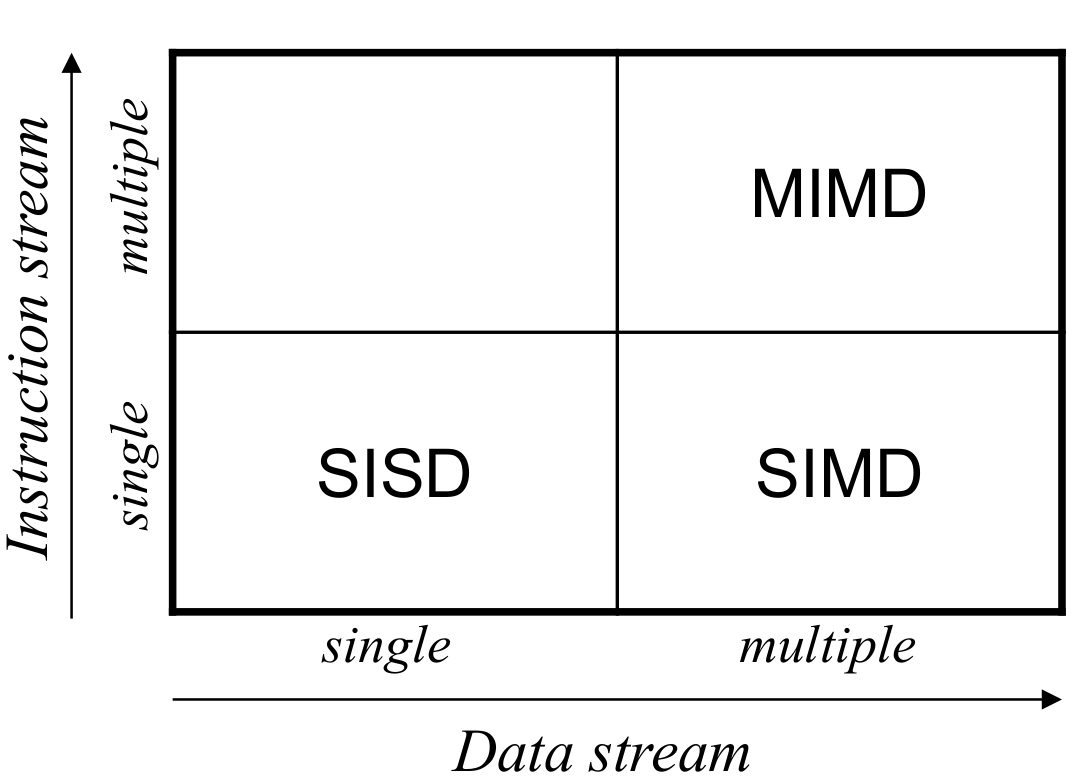
\includegraphics[scale=0.28]{flynns-taxonomy.png}
	\caption{
		Visualization of Flynn's Taxonomy \parencite[see][p5]{internet1}.
	}
	\label{fig:flynnsTax}
\end{figure}


\newpage

\subsection{Types of Parallelism}\label{subchap:typesOfParallelism}

Parallel computing is used for multiple processing elements simultaneously to solve any type of problem, as it's already explained in [\ref{chap:parallelCompArch}].

The Parallel Computing is evolved from serial computing that attempts to emulate what has always been the state of affairs in natural World.
Advantages of Parallel Computing over Serial Computing:
\begin{enumerate}
			\item {It saves time and money as many resources working together will reduce the time and cut potential costs.}
			\item {It can be impractical to solve larger problems on Serial Computing.}
			\item {It can take advantage of non-local resources when the local resources are finite.}
			\item {Serial Computing ‘wastes’ the potential computing power, thus Parallel Computing makes better work of hardware.}
\end{enumerate}

\noindent Beside the advantages for parallel computing, the different types of Parallelism are listed as the followings:

\begin{enumerate}
	 \item {\textbf{Bit-level parallelism}: This form of parallelism computing have it's roots based in the concept of increasing the processor's size. The amount of instructons it's reduced that the system must execute in order to perform a task on large-sized data.}
	 \item {\textbf{Instruction-level parallelism}: This form of parallelism computing is designed for a processor to only address less than one instruction for each clock cycle phase. The instructions can be re-ordered and grouped which are later on executed concurrently without affecting the result of the program.}
	  \item {\textbf{Task/Thread parallelism}: This form of parallelism computing is designed to employ the subtasks fragments of a decompositioned task and then allocate the fragments subtasks for execution concurrently} \parencite{book7}.
\end{enumerate}   

\noindent \textbf{Thread-level parallelism} is the only way to execute independent programs or discrete parts of a single program, simultaneously, using different sources of execution, like multiple processors sharing code, data and most of their address space, which are called threads.
 
In these days the term thread is often used in a casual way to refer to multiple executions that may run on different processors, even if they don't share an address space. To take advantage of an MIMD multiprocessor with n processors, we must usually have at least n threads or processes to execute. The independent threads are typically identified by the programmer or created by the compiler. Since the parallelism in this situation is contained in the threads, it is called thread-level parallelism. This corresponding architectural organization is also called chip multiprocessing (CMP). An example for CMP is the placement of multiple independent execution cores with all execution resources onto a single processor chip. The resulting processors are called multicore processors.

An alternative approach is the use of multithreading to execute multiple threads simultaneously ona single processor by switching between the different threads when needed by the hardware \parencite{internet9}.

\section{Parallel Programming Models}\label{chap:parPrgModels}

A parallel programming model is defined as a set of program abstractions which helps application's parallel activities to fit to the underlying parallel hardware, spanning over layers like programming languages, compilers, libraries, network communications and input/output systems.

Two widely known parallel programming models are shared memory and message passing, but there are also different combinations of both.

In the {\textbf{shared memory} programming model, threads share a common address space, which they read and write in an asynchronous manner. The concept represents a semaphore or lock that is used for synchronization, when the situation that more than one thread accesses the same data variable, the semaphore keeps data local to the processor and makes private copies avoiding expensive memory accesses. In the case of multiple processors sharing the same data with writing possibility, it needs some mechanisms of coherence maintenance.
	
In the {\textbf{message passing} programming model, threads used to communicate via message exchange having private memories. For message exchanging, each sends operation needs to have a corresponding receive operation. Threads are not constrained to exist on te same physical machine. 
	
A suitable mixture of these two models is appropriate. Processors can directly access memory on another processor. This is achieved via message passing, but what the programmer actually sees is shared-memory model.

\subsection{Classification of Parallel Programming Models}

In general, models for parallel programming are distinguished according to their abstraction levels \parencite{book1}. Therefore, the models are basically divided into four different classes:

\begin{enumerate}
	\item \underline{Machine model}:
	
	This model describes the lowest level of abstraction, in which the hardware description, the operating system, registers or input and output buffers are pointed out \parencite[see][p105]{book1}. 
	
	\item \underline{Architectural models}:
	
	The next level of abstraction are the architectural models. In this kind of model, the ``\textit{interconnection network of parallel platforms, the memory organization, the synchronous or asynchronous processing, or the execution mode of single instructions by SIMD or MIMD}'' \parencite[see][p105-106]{book1} are described.
	
	\item \underline{Computational model}:
	
	The model of computation is based on cost functions and a more formal model of a ``\textit{corresponding architectural model}'' \parencite[see][p106]{book1}. It also takes execution time along side with the providing of resources regarding to an architectural model into account \parencite{book1}. Analytical methods for designing and evaluating algorithms are also part of this model to quantify proper computations as we already mentioned in Chapter \ref{chap:mathComp}.
	
	\newpage
	
	\item \underline{Programming model}:
	
	The highest level of abstraction is the programming model.
	A description here is based on ``\textit{the semantics of the programming language or programming environment}'' \parencite[see][p106]{book1} to specify parallel programs. Therefore, a computation is mainly separated into ``\textit{(i) a sequence of instructions performing arithmetic or logical operations, (ii) a sequence of statements where each statement may capture several instructions, or (iii) a function or method invocation which typically consists of several statements}'' \parencite[see][p106]{book1}.
\end{enumerate}

\noindent Based on the different types of models, two major group of model classification should also be discussed.

\subsubsection{Process Interaction}

Non independent parallel computations need synchronization and communication to exchange data or for notification purposes. The model of process interaction wants to provide possibilities to deal with that kind of problem \parencite[see][p4]{internet1}. In general, we distinguish between three different process interaction models: the first one is called Shared address space programming (shared memory) \parencite{internet1}. In this model, parallel processes are able to share data asynchronously through a global address space. In this case, the programmer has to aware of race conditions, when two processes want to have access to the same resource. In this case mutex, semaphore or locks are used.

The second one is the Message Passing model. It describes a point to point connection between two tasks, to ensure synchronously ore asynchronously communication. The aim of this programming model is to point out the ability to invoke code to run not by calling a function, rather than by a process.

Performing parallelism is also possible by compiler. In this case, not the programmer is responsible for the implementation itself. Regarding to the used programming language or the provided functions, parallelism will be achieved by an intelligent compiling process. This model is also known as Implicit Interaction \parencite{internet1}.

\subsubsection{Problem decomposition}

In comparison to process interaction, problem decomposition provides independent parallel execution. Generally, three different types of models have to be discussed. First of all, as we already mentioned in Chapter \ref{subchap:typesOfParallelism}, task parallelism describes the basic method of threads, which contains assets of instructions or data. In addition to that, Flynn's Taxonomy usually classified this type of model as MIMD/MPMD or MISD [see Chapter \ref{subchap:flynnsTax}]. 

In contrast to that, data parallelism focus on processing different sections of data, e.g. an array of elements [see Chapter \ref{chap:mathComp}]. Processing the data will be independent, so therefore no race conditions appear. Flynn's Taxonomy classified this type of model as MIMD/SPMD or SIMD [see Chapter \ref{subchap:flynnsTax}].

Implicit parallelism is comparable to Implicit Interaction. The compiler and/or the hardware during runtime is responsible for parallelism. This can be achieved by translating serial into parallel code or by instruction-level parallelism [see Chapter \ref{subchap:typesOfParallelism}].